\documentclass[11pt,a4paper]{report}

% Aberstwyth dissertation LaTeX Template
% Authors: Dr. Hannah Dee (hmd1@aber.ac.uk), Neil Taylor (nst@aber.ac.uk)
% This has been adapted from the Leeds Thesis template and the
% Group Project template for Computer Science in Aberystywth University.
%
% All comments and suggestions welcome.
%
% Template designed to be used with pdflatex: it may need alteration to
% run with a different LaTeX engine.
%
% Note - this is offered as a starting point for your work. You are not
% required to use this template and can choose to create your own document
% without it.

% To build document on the unix command line, run four commands:

% pdflatex dissertation
% bibtex dissertation
% pdflatex dissertation
% pdflatex dissertation

% you will end up with dissertation.pdf
\usepackage{mmp}
\usepackage{pdfpages}

% the following packages are used for citations - You only need to include one.
%
% Use the cite package if you are using the numeric style (e.g. IEEEannot).
% Use the natbib package if you are using the author-date style (e.g. authordate2annot).
% Only use one of these and comment out the other one.
% \usepackage{cite}
%\usepackage{natbib}

% Use the following to selectively exclude chapters
%\includeonly{cover,abstract,acknowledge,declare,chapter1,chapter2}

\begin{document}

% all of the include directives below refer to tex files
% so 
\title{Quiz Tool}

% Your name
\author{Mr. Michal Goly}

% Your email
\authoremail{mwg2@aber.ac.uk}

\degreeschemecode{G600} %e.g. G400
\degreeschemetitle{Software Engineering} % e.g. Computer Science
\degreetype{BEng}

\modulecode{CS39440} % i.e. CS39440, CC39440, CS39620
\moduletitle{Major Project} % i.e. Major Project or Minor Project

\date{18th April 2017} % i.e. the date of this version of the report

\status{Draft} % Use draft until you create the release version. Then, change this to Release.
\version{1.1}

%The title and name of your supervisor.
\supervisor{Mr. Chris Loftus}

%The email for your supervisor.
\supervisoremail{cwl@aber.ac.uk}

\maketitle
 includes cover.tex - to change the content,
% edit the tex file

\pagenumbering{roman}

% This is the front page

\title{Quiz Tool}

% Your name
\author{Mr. Michal Goly}

% Your email
\authoremail{mwg2@aber.ac.uk}

\degreeschemecode{G600} %e.g. G400
\degreeschemetitle{Software Engineering} % e.g. Computer Science
\degreetype{BEng}

\modulecode{CS39440} % i.e. CS39440, CC39440, CS39620
\moduletitle{Major Project} % i.e. Major Project or Minor Project

\date{18th April 2017} % i.e. the date of this version of the report

\status{Draft} % Use draft until you create the release version. Then, change this to Release.
\version{1.1}

%The title and name of your supervisor.
\supervisor{Mr. Chris Loftus}

%The email for your supervisor.
\supervisoremail{cwl@aber.ac.uk}

\maketitle


% Set up page numbering
\pagestyle{empty}

% declarations of originality
\thispagestyle{empty}

%%%
%%% You must sign the declaration of originality. 
%%%
%%% You are submitting this electronically. Therefore, to sign, you 
%%% type your name and date to replace the .... characters. 
%%%
\begin{center}
    {\LARGE\bf Declaration of originality}
\end{center}

I confirm that:

\begin{itemize}
\item{This submission is my own work, except where 
clearly indicated.}

\item{I understand that there are severe penalties for Unacceptable Academic Practice, which can lead to loss of marks or even the withholding of a degree.}
 
\item{I have read the regulations on Unacceptable Academic Practice from the University's Academic Quality and Records Office (AQRO) and the relevant sections of the current Student Handbook of the Department of Computer Science.}
 
\item{In submitting this work I understand and agree to abide by the University's regulations governing these issues.}
\end{itemize}

\vspace{2em}
Name ............................................................  \\

\vspace{1em}
Date ............................................................ \\

%%% 
%%% We would like to make a selection of final reports available to students that take 
%%% this module in future years. To enable us to do this, we require your consent. You 
%%% are not required that you do this, but if you do give your consent, then we will have 
%%% the option to select yours as one of a number of reports as examples for other 
%%% students. If you would like to give your consent, then please include the following 
%%% text and type your name and date to replace the .... characters. 
%%% 
%%% If you do not wish to give your consent, please remove this from your report. 
%%%
\vspace{1em}
\begin{center}
    {\LARGE\bf Consent to share this work}
\end{center}

By including my name below, I hereby agree to this dissertation being made available to other students and academic staff of the Aberystwyth Computer Science Department.  

\vspace{2em}
Name ............................................................  \\

\vspace{1em}
Date ............................................................ \\




\thispagestyle{empty}

\begin{center}
    {\LARGE\bf Acknowledgements}
\end{center}

I am grateful to coffee.
 % Acknowledgements
\thispagestyle{empty}

\begin{center}
    {\LARGE\bf Abstract}
\end{center}
Student engagement and live knowledge monitoring are vital in the provision of good quality
lecture content in 2018. It is important to make sure audience understands concepts presented,
and quizzes can help lecturers judge students' understanding in real time.

Aberystwyth University currently uses Qwizdom\cite{1} live polling tool during the provision
of some lectures and practical sessions. The university operates under a single license
forcing lecturers to book sessions before they can use the tool. Due to human nature,
session hijacking occasionally occurs to the bemusement of both students and lecturers.
For example, students could be shown biology slides half way through their geography
lecture.

This project focused on the design and development of an in-house built Quiz Tool,
enabling multiple lecturers to use it at the same time and potentially making Qwizdom
redundant in the future. This ambition could only be achieved if the project was of
high quality and its future maintainability was considered at all stages of the design
and development.

The Quiz Tool allows lecturers to login using their Google Single Sign-on\cite{2} credentials,
upload their PDF lecture slides and create \textit{Lectures} in the system.
Each \textit{Lecture} can be then edited, and eligible slides can be marked as quizzes.
True/false, single and multi choice style quizzes are supported. Once a lecturer is happy with their
\textit{Lecture}, he can broadcast it and receive a session key which can be
shared with students. Lecture slides will be shown to all students and the
lecture can be delivered in a traditional fashion up to the moment a slide has been marked as a quiz.
Students will then be able to answer
the question and polling results will be presented in real time to the lecturer.
Lecture sessions broadcasted in the past are kept, and students' answers can be exported
as a PDF report for future analysis.

The tool is composed of a back-end with an associated database, and two
front-ends. One for lecturers and one for students. Finally, the tool has been
successfully developed using an agile methodology, adjusted for a single person
project.
                 % Abstract

\pagenumbering{roman}
\pagestyle{fancy}
\fancyhead{}
\fancyfoot[C]{\thepage}
\renewcommand{\headrulewidth}{0 pt}
\renewcommand{\chaptermark}[1]{\markboth{#1}{}}

\tableofcontents
\newpage
\listoffigures
\newpage
\listoftables
\newpage

% Set up page numbering
\pagenumbering{arabic}

\setchapterheaderfooter

% include the chapters
\chapter{Background \& Objectives}

% This section should discuss your preparation for the project, including background
% reading, your analysis of the problem and the process or method you have followed
% to help structure your work.  It is likely that you will reuse part of your outline
% project specification, but at this point in the project you should have more to talk about.

\section{Background}
% What was your background preparation for the project? What similar systems did
% you assess? What was your motivation and interest in this project?

\subsection{Motivation}
I enjoy programming, and this project seemed to involve a lot of coding. I was also excited
to build a complex, real time system, while applying my previous software engineering
experience and learning new technologies at the same time. I knew I would be given
a lot of freedom to choose the most appropriate tools for the task, and incorporate
modern software development practices, including continuous integration and
containerised environments, to deliver good quality software. I was also keen on developing something that could be actually
useful to the university once I leave Aberystwyth. It is more motivating to develop
a product, while knowing it could be potentially used in real life, as opposed to being
forgotten after the submission. I have experienced being presented with wrong slides
during a lecture in my first year at university, so I was happy to address the problem
of a single session Qwizdom license with my tool.

\subsection{Technology Considerations}
\subsubsection{Programming Languages}
% - Initial proposal to create an Android based system for students -> React Native -> MEAN
The initial proposal was to create the classroom quiz system using Java\cite{3} to run it natively
on Android\cite{4} mobile devices. The lecturer was supposed the create quizzes on his teaching
machine, by interacting with the system using a web front end. Lecture slides were then supposed
to be broadcasted to his audience, and they could use their mobile phones to answers questions,
which would be then sent back to the lecturer for analysis. I have had previous experience with
native Android development, therefore this approach seemed like a reasonable option. The only problem was,
iOS\cite{5} devices are very popular in the United Kingdom, and developing an app for Android would exclude
a good percentage of students from being able to actively participate in lectures presented. I have
therefore started to think about alternative approaches.

The second possibility was to use React Native\cite{6}, a JavaScript\cite{7} framework allowing
developers to create mobile applications in JavaScript and compile it down to both iOS and Android.
This approach would still require the web front end for the lecturer to be developed, and a natural
choice would be to use React\cite{8} to keep the learning curve as low as possible.

The final alternative considered, was to develop the whole tool as a web application. This way both the
front end for lecturers and students could be developed using the same framework. Members of the audience
could participate in lectures by accessing the web application using web browsers installed
both on their mobile phones, regardless of the operating system, or even their laptops. I considered
both React and Angular 4\cite{9}, since I have already briefly used it before. React is a library
for developing user interface, whereas Angular is a web development framework. The only caveat with
using Angular is that the developer needs to learn TypeScript\cite{10}, which compiles down to JavaScript.

\subsubsection{The WebSocket Protocol}
The Quiz Tool was supposed to allow a lecturer to broadcast his slides to all the students
participating in a lecture. This requires a bidirectional communication protocol between the
server and the clients. For example, if a lecturer emits the next slide of his presentation,
this change should be pushed to the back end, and then the back end needs to be able to
send the new slide to all the students. Students' clients should also be able to push quiz
answers back to the back end, so they can be presented to the lecturer in some form.

The WebSocket Protocol can be used to create such real time systems. It enables two-way
communication between a client and a remote host, making it ideal for instant messaging,
gaming applications, and the Quiz Tool. It uses a single TCP connection for trafic
in both directions\cite{11}.

\subsubsection{Prototyping}
I have followed various tutorials to quickly prototype proof of concept applications,
in order to learn more about the technologies which could be useful during the Quiz Tool
development. I started with the Socket.io chat tutorial. Socket.io is
a JavaScript library enabling bidirectional event-based communication, and uses
the WebSocket Protocol internally\cite{12}. I have created a chat application following one
of the tutorials on their homepage\cite{13}. I have also learned the basics of
Angular by following the Tour of Heroes tutorial\cite{14}, and finally tried to
understand how Angular could work together with Socket.io by following the MEAN
Socket.io tutorial\cite{15}.

\subsection{Similar Tools}
- Qwizdom

\subsection{Internal vs External Hosting}
- local LSX container vs external cloud provider -> LDAP

\section{Analysis}
% Taking into account the problem and what you learned from the background work,
% what was your analysis of the problem? How did your analysis help to decompose
% the problem into the main tasks that you would undertake? Were there alternative
% approaches? Why did you choose one approach compared to the alternatives?
%
% There should be a clear statement of the objectives of the work, which you will
% evaluate at the end of the work.
%
% In most cases, the agreed objectives or requirements will be the result of a compromise
% between what would ideally have been produced and what was determined to be possible in
%  the time available. A discussion of the process of arriving at the final list is usually appropriate.
%
% As mentioned in the lectures, think about possible security issues for the project topic.
%  Whilst these might not be relevant for all projects, do consider if there are relevant
%   for your project. Where there are relevant security issues, discuss how they will
%   this affect the work that you are doing. Carry forward this discussion into relevant
%    areas for design, implementation and testing.
- MEAN stack \& Docker \& docker-compose
- Version Control
- build - Circle CI -> testing, autodeploy
- AWS Production environment (did not know of Elasticbeanstalk at this point)
- Google Single Sign On -> Security
- Identification of major problems
- Top level requirements of the system


\section{Process}
% You need to describe briefly the life cycle model or research method that you used. You
%  do not need to write about all of the different process models that you are aware of.
%  Focus on the process model that you have used. It is possible that you needed to adapt
%  an existing process model to suit your project; clearly identify what you used and how
%  you adapted it for your needs.

%\addcontentsline{toc}{chapter}{Development Process}
\chapter{Design}

You should concentrate on the more important aspects of the design. It is essential that an overview is presented before going into detail. As well as describing the design adopted it must also explain what other designs were considered and why they were rejected.

The design should describe what you expected to do, and might also explain areas that you had to revise after some investigation.

Typically, for an object-oriented design, the discussion will focus on the choice of objects and classes and the allocation of methods to classes. The use made of reusable components should be described and their source referenced. Particularly important decisions concerning data structures usually affect the architecture of a system and so should be described here.

How much material you include on detailed design and implementation will depend very much on the nature of the project. It should not be padded out. Think about the significant aspects of your system. For example, describe the design of the user interface if it is a critical aspect of your system, or provide detail about methods and data structures that are not trivial. Do not spend time on long lists of trivial items and repetitive descriptions. If in doubt about what is appropriate, speak to your supervisor.
 
You should also identify any support tools that you used. You should discuss your choice of implementation tools - programming language, compilers, database management system, program development environment, etc.

Some example sub-sections may be as follows, but the specific sections are for you to define. 

\section{Overall Architecture}

\section{Some detailed design}

\subsection{Even more detail}

\section{User Interface}

\section{Other relevant sections}
\chapter{Implementation}

The implementation should look at any issues you encountered as you tried to implement your design. During the work, you might have found that elements of your design were unnecessary or overly complex; perhaps third party libraries were available that simplified some of the functions that you intended to implement. If things were easier in some areas, then how did you adapt your project to take account of your findings?

It is more likely that things were more complex than you first thought. In particular, were there any problems or difficulties that you found during implementation that you had to address? Did such problems simply delay you or were they more significant?

You can conclude this section by reviewing the end of the implementation stage against the planned requirements. 

% add any additional chapters here

\setemptyheader
% start the appendix - sets up different numbering
\fancypagestyle{plain}{%
%\fancyhf{} % clear all header and footer fields
\fancyhead[L]{\textsl{Appendix\ \thechapter}}
\fancyhead[R]{\textsl{\leftmark}}}

\appendix
\fancyhead[L]{\textsl{Appendix\ \thechapter}}
\fancyhead[R]{\textsl{\leftmark}}
\fancyhead[C]{}
\fancyfoot[C]{\thepage}
\renewcommand{\headrulewidth}{0.4pt}
\renewcommand{\chaptermark}[1]{\markboth{#1}{}}

\fancyhead[L]{\textsl{Appendix\ \thechapter}}
\fancyhead[R]{\textsl{\leftmark}}
\fancyfoot[C]{{\thepage} of \pageref{LastPage}}

% include any appendices here
\chapter{Third-Party Code and Libraries}
%
% If you have made use of any third party code or software libraries, i.e. any code
% that you have not designed and written yourself, then you must include this appendix.
%
% As has been said in lectures, it is acceptable and likely that you will make use of
%  third-party code and software libraries. If third party code or libraries are used,
%   your work will build on that to produce notable new work. The key requirement is that we
%   understand what is your original work and what work is based on that of other people.
%
% Therefore, you need to clearly state what you have used and where the original material can be
% found. Also, if you have made any changes to the original versions, you must explain what you have changed.
%
% As an example, you might include a definition such as:
%
% Apache POI library - The project has been used to read and write Microsoft Excel files (XLS) as
%  part of the interaction with the client's existing system for processing data. Version 3.10-FINAL
%   was used. The library is open source and it is available from the Apache Software Foundation
% \cite{apache_poi}. The library is released using the Apache License
% \cite{apache_license}. This library was used without modification.

% server package.json
\subparagraph{body-parser v1.18.2}
MIT licensed Node.js middleware for parsing bodies of incoming HTTP requests. Used as part of the
\texttt{server\_node} container. [Online] Available: https://github.com/expressjs/body-parser, [Accessed: Apr. 20, 2018].

\subparagraph{express v4.15.2}
MIT licensed Node.js web development framework used to develop the back end of the Quiz Tool.
[Online] Available: https://github.com/expressjs/body-parser, [Accessed: Apr. 20, 2018].

\subparagraph{eyes v0.1.8}

\subparagraph{fs v0.0.1-security}
\subparagraph{jsonschema v1.2.2}
\subparagraph{mongoose v5.0.7}
\subparagraph{multer v1.3.0}
\subparagraph{passport v0.4.0}
\subparagraph{passport-google-oauth v1.0.0}
\subparagraph{pdf-extract v1.0.11}
\subparagraph{pdf2img v0.5.0}
\subparagraph{request-promise v4.2.2}
\subparagraph{request v2.83.0}
\subparagraph{socket.io v2.0.4}
\subparagraph{mocha v5.0.4}
\subparagraph{chai v4.1.2}
\subparagraph{chai-http v3.0.0}
\subparagraph{selenium-webdriver v4.0.0-alpha.1}

% server Dockerfile
\subparagraph{ghostscript}
\subparagraph{poppler-utils}
\subparagraph{pdftk}
\subparagraph{graphicsmagick}

% client package.json
\subparagraph{@angular/animations v4.4.4}
\subparagraph{@angular/common v4.3.5}
\subparagraph{@angular/compiler v4.3.5}
\subparagraph{@angular/core v4.3.5}
\subparagraph{@angular/forms v4.3.5}
\subparagraph{@angular/http v4.3.5}
\subparagraph{@angular/platform-browser v4.3.5}
\subparagraph{@angular/platform-browser-dynamic v4.3.5}
\subparagraph{@angular/router v4.3.5}
\subparagraph{@types/jspdf v1.1.31}
\subparagraph{@types/socket.io-client v1.4.32}
\subparagraph{chart.js v2.7.2}
\subparagraph{file-saver v1.3.8}
\subparagraph{core-js v2.5.0}
\subparagraph{font-awesome v4.7.0}
\subparagraph{intl v1.2.5}
\subparagraph{jspdf v1.3.5}
\subparagraph{jspdf-autotable v2.3.2}
\subparagraph{mdi v2.1.19}
\subparagraph{ng2-charts v1.6.0}
\subparagraph{ng2-file-upload v1.3.0}
\subparagraph{ng2-materialize v1.8.0}
\subparagraph{ngx-cookie-service v1.0.10}
\subparagraph{rxjs v5.4.3}
\subparagraph{socket.io-client v2.0.4}
\subparagraph{zone.js v0.8.16}
\subparagraph{@angular/cli v1.3.1}
\subparagraph{@angular/compiler-cli v4.3.5}
\subparagraph{@types/jasmine v2.5.38}
\subparagraph{codelyzer v3.1.2}
\subparagraph{jasmine-core v2.5.2}
\subparagraph{jasmine-spec-reporter v3.2.0}
\subparagraph{karma v1.4.1}
\subparagraph{karma-cli v1.0.1}
\subparagraph{karma-coverage-istanbul-reporter v0.2.0}
\subparagraph{karma-jasmine v1.1.0}
\subparagraph{karma-jasmine-html-reporter v0.2.2}
\subparagraph{karma-phantomjs-launcher v1.0.4}
\subparagraph{protractor v5.1.0}
\subparagraph{ts-node v3.3.0}
\subparagraph{tslint v5.6.0}
\subparagraph{typescript v2.4.2}

% tutorials
\subparagraph{Building Chat Application using MEAN Stack (Angular 4) and Socket.io}
Step by step tutorial of building a simple chat application using MEAN stack and Socket.io. It helped me
to understand how to use MEAN with Socket.io together, and the initial structure of the application
was inspired by it.
[Online] Available: https://www.djamware.com/post/58e0d15280aca75cdc948e4e/building-chat-applicationusing-mean-stack-angular-4-and-socketio,
[Accessed: Apr. 11, 2018].

\subparagraph{Docker Compose | Containerizing MEAN Stack Application | DevOps Tutorial | Edureka}
A YouTube tutorial explaining how to containerise a MEAN stack web application. The \texttt{docker-compose.yml}
file has been based on the one showed in the video. [Online] Available: https://www.youtube.com/watch?v=WZa7GsqyS3w,
[Accessed: Apr. 20, 2018].

\subparagraph{Dockerized Angular 4 App (with Angular CLI)}
MIT licensed GitHub repository showing a starter Angular application, containerised with nginx
using Docker. The structure of \texttt{client} container is based on a fork of the repository.
[Online] Available: https://github.com/avatsaev/angular4-docker-example, [Accessed: Apr. 20, 2018].

\subparagraph{Multicontainer Docker Environments}
An official AWS tutorial showing how to deploy an application to the Multicontainer Elasticbeanstalk Docker
Environment. [Online] Available: https://docs.aws.amazon.com/elasticbeanstalk/latest/dg/create\_deploy\_docker\_ecs.html, [Accessed: Apr. 20, 2018].

\subparagraph{Test a Node RESTful API with Mocha and Chai}
A tutorial showing how to tests Node.js applications with Mocha and Chai. The structure of the server side
unit tests has been inspired by the tutorial. [Online] Available: https://scotch.io/tutorials/test-a-node-restful-api-with-mocha-and-chai,
[Accessed: Apr. 20, 2018].

\subparagraph{MEAN with Angular 2/5 - User Registration and Login Example \& Tutorial}
The authentication of the Quiz Tool has been inspired by this tutorial. Especially the Angular
JWT interceptor used in the application to append authentication tokens to each HTTP requests is based on the
code presented in the tutorial. [Online] Available: http://jasonwatmore.com/post/2017/02/22/mean-with-angular-2-user-registration-and-login-example-tutorial,
[Accessed: Apr. 20, 2018].

\subparagraph{6 16 integrating with google oauth with passport js in a MEAN app undergrad webdev summer 1 2017}
A YouTube tutorial explaining how to configure google authentication with the passport Node.js
authentication middleware, in a MEAN stack application. The Google Sign-In implemented in Quiz Tool
has been based on this tutorial. [Online] Available: https://www.youtube.com/watch?v=rc6zYV4jShQ,
[Accessed: Apr. 20, 2018].

\subparagraph{How to setup Elastic Beanstalk Deployment?}
A topic in the official Circle CI discussion forum describing how to setup Circle CI to automatically
deploy to the Elastic Beanstalk environment hosted on AWS. [Online] Available: https://discuss.circleci.com/t/how-to-setup-elastic-beanstalk-deployment/6154/4,
[Accessed: Apr. 20, 2018].

\subparagraph{Getting Started with Docker Compose}
A step-by-step introduction to using the official Selenium Docker images using docker-compose. The tutorial
was used when integration selenium tests were added to test the application.
[Online] Available: https://github.com/SeleniumHQ/docker-selenium/wiki/Getting-Started-with-Docker-Compose,
[Accessed: Apr. 20, 2018].










%


\chapter{Ethics Submission}

Ethics Application Number: 9563

\includepdf[pages=-]{Appendix2/9563.pdf}

\chapter{Code Examples}

For some projects, it might be relevant to include some code extracts in an appendix. You are not expected to put all of your code here - the correct place for all of your code is in the technical submission that is made in addition to the Final Report. However, if there are some notable aspects of the code that you discuss, including that in an appendix might be useful to make it easier for your readers to access. 

As a general guide, if you are discussing short extracts of code then you are advised to include such code in the body of the report. If there is a longer extract that is relevant, then you might include it as shown in the following section. 

Only include code in the appendix if that code is discussed and referred to in the body of the report. 

\section{Random Number Generator}

The Bayes Durham Shuffle ensures that the psuedo random numbers used in the simulation are further shuffled, ensuring minimal correlation between subsequent random outputs \cite{NumericalRecipes}.

\begin{verbatim}
 #define IM1 2147483563
 #define IM2 2147483399
 #define AM (1.0/IM1)
 #define IMM1 (IM1-1)
 #define IA1 40014
 #define IA2 40692 
 #define IQ1 53668
 #define IQ2 52774
 #define IR1 12211
 #define IR2 3791
 #define NTAB 32
 #define NDIV (1+IMM1/NTAB)
 #define EPS 1.2e-7
 #define RNMX (1.0 - EPS)
 
 double ran2(long *idum)
 {
   /*---------------------------------------------------*/
   /* Minimum Standard Random Number Generator          */
   /* Taken from Numerical recipies in C                */
   /* Based on Park and Miller with Bays Durham Shuffle */
   /* Coupled Schrage methods for extra periodicity     */
   /* Always call with negative number to initialise    */
   /*---------------------------------------------------*/	
 
   int j;
   long k;
   static long idum2=123456789;
   static long iy=0;
   static long iv[NTAB];
   double temp;
 
   if (*idum <=0)
   {
     if (-(*idum) < 1)
     {
       *idum = 1;
     }else
     {
       *idum = -(*idum);
     }
     idum2=(*idum);
     for (j=NTAB+7;j>=0;j--)
     {
       k = (*idum)/IQ1;
       *idum = IA1 *(*idum-k*IQ1) - IR1*k;
       if (*idum < 0)
       {
         *idum += IM1;
       }
       if (j < NTAB)
       {
         iv[j] = *idum;
       }
     }
     iy = iv[0];	
   }
   k = (*idum)/IQ1;
   *idum = IA1*(*idum-k*IQ1) - IR1*k;
   if (*idum < 0)
   {
     *idum += IM1;
   }
   k = (idum2)/IQ2;
   idum2 = IA2*(idum2-k*IQ2) - IR2*k;
   if (idum2 < 0)
   {
     idum2 += IM2;
   }
   j = iy/NDIV;
   iy=iv[j] - idum2;
   iv[j] = *idum;
   if (iy < 1)
   {
     iy += IMM1;
   }
   if ((temp=AM*iy) > RNMX)
   {
     return RNMX;
   }else
   {
     return temp;	
   }
 }
 
\end{verbatim}


\chapter{Sprint Retrospective Documents}
\label{chap:spintretrospectives}

This appendix contains the sprint retrospective documents produced at the end
of each sprint.

\includepdf[pages=-]{Appendix4/1.pdf}
\includepdf[pages=-]{Appendix4/2.pdf}
\includepdf[pages=-]{Appendix4/2_5.pdf}
\includepdf[pages=-]{Appendix4/3.pdf}

\chapter{Code Examples}
\label{chap:codesamples}

This appendix contains code examples relevant to the discussion in the main body of the
report.

\newpage
\section{Intial Front End Dockerfile}
The initial \texttt{Dockerfile} of the client container added in the first sprint of
the development of the tool.

\begin{figure}[ht]
  \begin{lstlisting}[basicstyle=\small, breaklines=true]
    ### STAGE 1: Build ###

    # We label our stage as 'builder'
    FROM node:8-alpine as builder

    COPY package.json package-lock.json ./

    RUN npm set progress=false && npm config set depth 0 && npm cache clean --force

    ## Storing node modules on a separate layer will prevent unnecessary npm installs at each build
    RUN npm i && mkdir /ng-app && cp -R ./node_modules ./ng-app

    WORKDIR /ng-app

    COPY . .

    ## Build the angular app in production mode and store the artifacts in dist folder
    RUN $(npm bin)/ng build --prod --build-optimizer

    ### STAGE 2: Setup ###

    FROM nginx:1.13.3-alpine

    ## Copy our default nginx config
    COPY nginx/default.conf /etc/nginx/conf.d/

    ## Remove default nginx website
    RUN rm -rf /usr/share/nginx/html/*

    ## From 'builder' stage copy over the artifacts in dist folder to default nginx public folder
    COPY --from=builder /ng-app/dist /usr/share/nginx/html

    CMD ["nginx", "-g", "daemon off;"]
  \end{lstlisting}
  \caption{Intial Front End Dockerfile}
  \label{sample:clientdocker}
\end{figure}

\newpage
\section{Initial Back End Dockerfile}
The initial \texttt{Dockerfile} of the server\_node container added in the first sprint of
the development of the tool.

\begin{figure}[h!]
    \begin{lstlisting}[basicstyle=\small]
    FROM node:carbon
    WORKDIR /usr/src/app
    COPY package*.json ./
    RUN npm install
    COPY . .
    EXPOSE 3000
    CMD [ "npm", "start" ]
  \end{lstlisting}
  \caption{Back End Dockerfile}
  \label{sample:serverdocker}
\end{figure}

\newpage
\section{Intial Circle CI Config File}
The initial \texttt{.circleci/config.yml} added in the first sprint of the development.

\begin{figure}[h!]
  \begin{lstlisting}[basicstyle=\small, breaklines=true]
  version: 2
  jobs:
    build:
      machine: true

      working_directory: ~/repo

      steps:
        - checkout

        - run:
            name: install docker-compose
            command: |
              set -x
              sudo chown -R $(whoami) /usr/local/bin
              curl -L https://github.com/docker/compose/releases/download/1.11.2/docker-compose-`uname -s`-`uname -m` > /usr/local/bin/docker-compose
              chmod +x /usr/local/bin/docker-compose

        - run:
            name: docker compose build image
            command: |
              set -x
              docker-compose build
              docker-compose up

        - run:
            name: unit tests
            command: |
              curl localhost

        # deploy only master branch
        - deploy:
            command: |
              if [ "${CIRCLE_BRANCH}" == "master" ]; then
                chmod +x scripts/deploy.sh
                ./scripts/deploy.sh
              fi
  \end{lstlisting}
  \caption{Initial Build Config File}
  \label{sample:circleci}
\end{figure}

\newpage
\section{Initial Dockerrun.aws.json file}
The initial version of the file specifying how containers should be linked together when running
in the production environment on AWS.

\begin{figure}[h!]
  \begin{lstlisting}[basicstyle=\small, breaklines=true]
  {
      "AWSEBDockerrunVersion": 2,
      "containerDefinitions": [
          {
              "name": "client",
              "image": "993389244112.dkr.ecr.eu-west-2.amazonaws.com/quiz-tool-client:latest",
              "memory": 128,
              "essential": true,
              "portMappings": [
                  {
                      "hostPort": 80,
                      "containerPort": 80
                  }
              ],
              "links": [
                  "server_node"
              ]
          },
          {
              "name": "server_node",
              "image": "993389244112.dkr.ecr.eu-west-2.amazonaws.com/quiz-tool-server:latest",
              "memory": 128,
              "essential": true,
              "links": [
                "database"
              ]
          },
          {
            "name": "database",
            "image": "mongo",
            "memory": 128,
            "essential": true,
            "portMappings": [
                {
                    "hostPort": 27017,
                    "containerPort": 27017
                }
            ]
          }
      ]
  }
  \end{lstlisting}
  \caption{Dockerrun.aws.json}
  \label{sample:dockerrunaws}
\end{figure}

\newpage
\section{Production Deployment Script}
The bash script performing the deployment from Circle CI to the production environment
hosted on AWS.

\begin{figure}[h!]
  \begin{lstlisting}[basicstyle=\small, breaklines=true]
  #!/bin/bash
  set -x
  set -e

  AWS_CONFIG_FILE=$HOME/.aws/config

  mkdir $HOME/.aws
  touch $AWS_CONFIG_FILE
  chmod 600 $AWS_CONFIG_FILE

  echo "[default]"                                     > $AWS_CONFIG_FILE
  echo "aws_access_key_id=$AWS_ACCESS_KEY_ID"         >> $AWS_CONFIG_FILE
  echo "aws_secret_access_key=$AWS_SECRET_ACCESS_KEY" >> $AWS_CONFIG_FILE

  $(aws ecr get-login --no-include-email --region eu-west-2)

  docker tag repo_client:latest 993389244112.dkr.ecr.eu-west-2.amazonaws.com/quiz-tool-client:latest
  docker tag repo_server_node:latest 993389244112.dkr.ecr.eu-west-2.amazonaws.com/quiz-tool-server:latest

  docker push 993389244112.dkr.ecr.eu-west-2.amazonaws.com/quiz-tool-client:latest
  docker push 993389244112.dkr.ecr.eu-west-2.amazonaws.com/quiz-tool-server:latest

  eb deploy prod-env
  \end{lstlisting}
  \caption{Production Deployment Script}
  \label{sample:deploy}
\end{figure}

\newpage
\section{Final Dockerrun.aws.json file}
The final version of the file specifying how Docker containers should be link with each other
when running in the production environment provided by AWS.
\begin{figure}[h!]
  \begin{lstlisting}[basicstyle=\tiny, breaklines=true]
{
    "AWSEBDockerrunVersion": 2,
    "volumes": [
      {
        "name": "mongo",
        "host": {
          "sourcePath": "/var/app/database"
        }
      }
    ],
    "containerDefinitions": [
        {
            "name": "client",
            "image": "993389244112.dkr.ecr.eu-west-2.amazonaws.com/quiz-tool-client:latest",
            "memory": 300,
            "essential": true,
            "portMappings": [
                {
                    "hostPort": 80,
                    "containerPort": 80
                }
            ],
            "links": [
                "server_node"
            ]
        },
        {
            "name": "server_node",
            "image": "993389244112.dkr.ecr.eu-west-2.amazonaws.com/quiz-tool-server:latest",
            "memory": 300,
            "essential": true,
            "links": [
              "database"
            ]
        },
        {
          "name": "database",
          "image": "mongo",
          "memory": 300,
          "essential": true,
          "mountPoints": [
              {
                "sourceVolume": "mongo",
                "containerPath": "/data/db"
              }
          ],
          "portMappings": [
              {
                  "hostPort": 27017,
                  "containerPort": 27017
              }
          ]
        }
    ]
}
\end{lstlisting}
\caption{Final Dockerrun.aws.json}
\label{sample:dockerrunawsfinal}
\end{figure}

\chapter{PDF Report Examples}
\label{chap:pdfreports}

This appendix contains examples of PDF reports generated with the Quiz Tool.

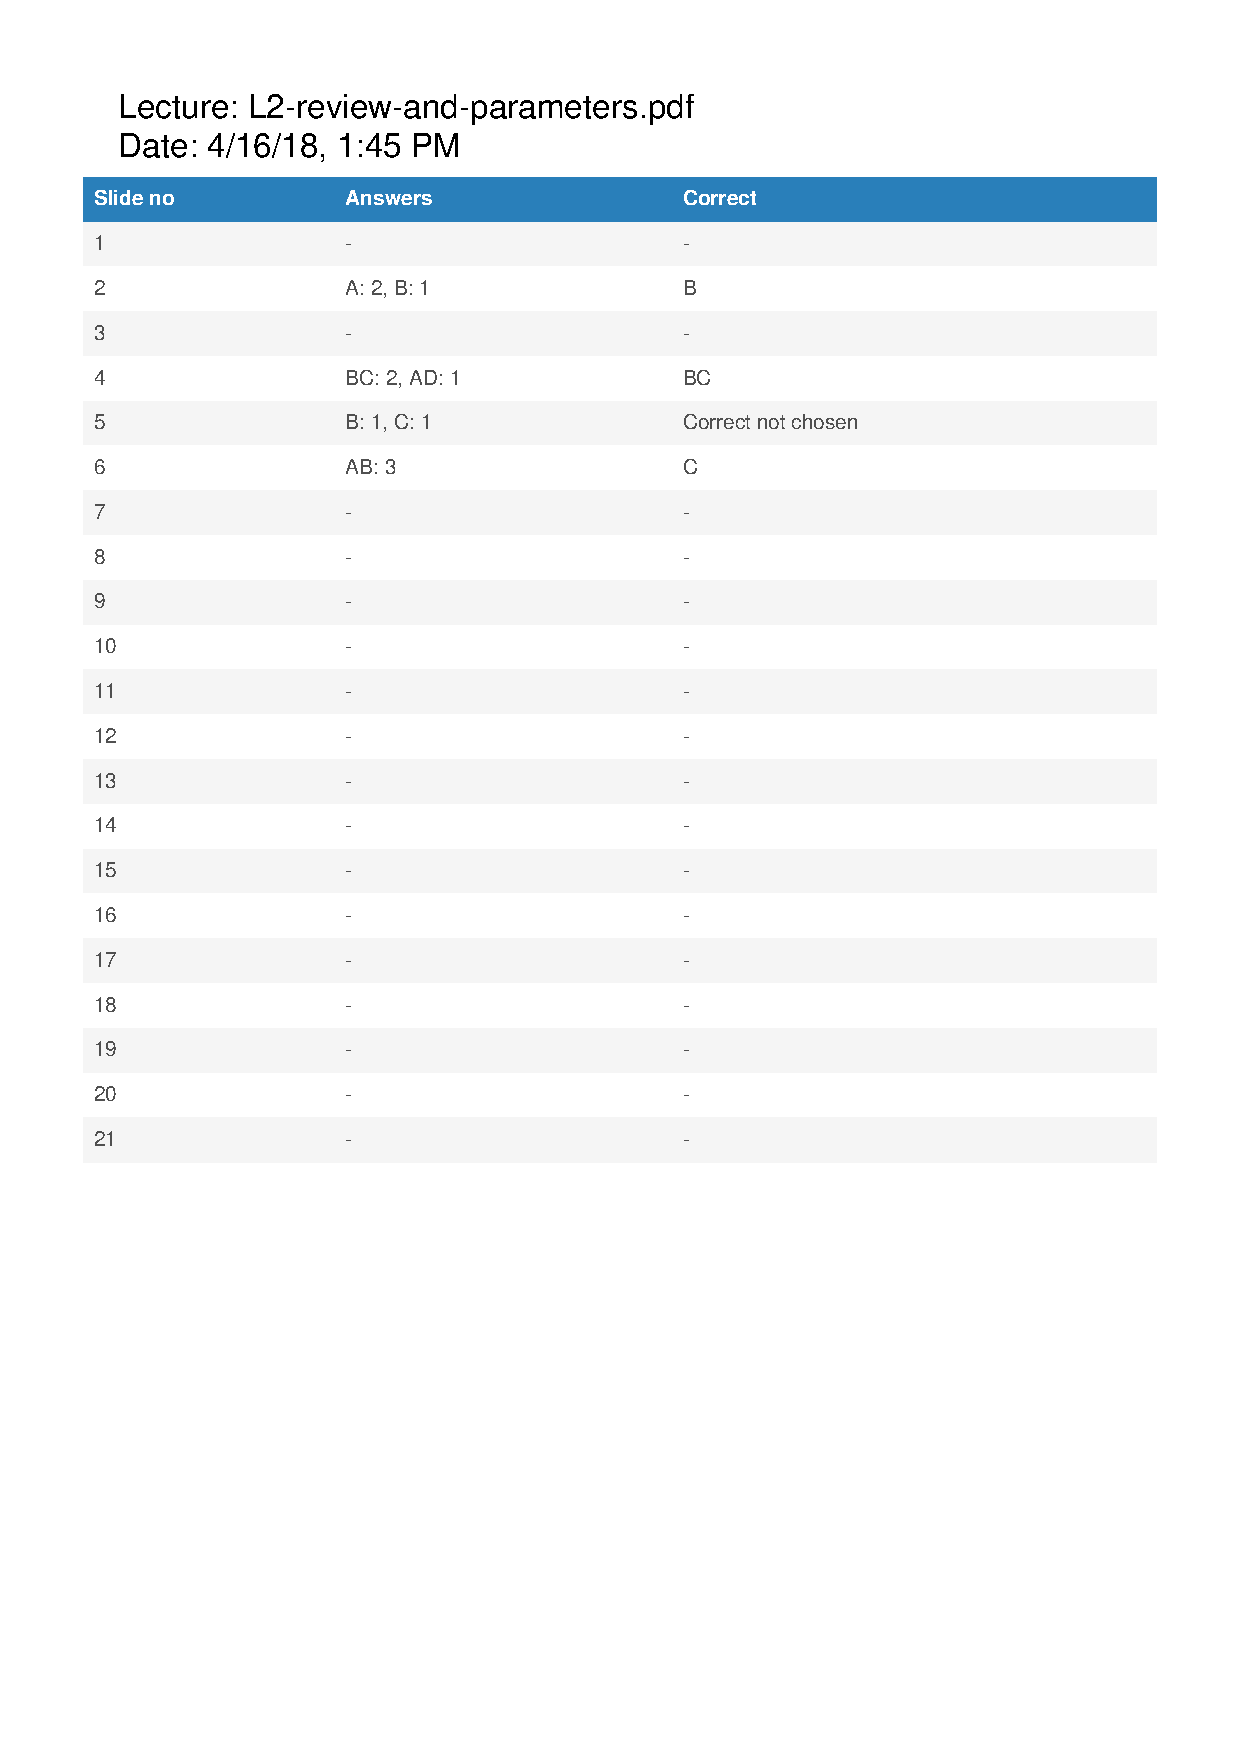
\includepdf[pages=-]{Appendix6/example.pdf}

\chapter{User Survey Results}
\label{chap:usersurvey}

This appendix contains raw responses from the user survey run after the Quiz
Tool has been used to run a real lecture with real students at Aberystwyth University.

\newpage
\begin{figure}[h!]
    \centering
    \includegraphics[width=\textwidth]{Appendix7/1.jpg}
    \caption{Question 1}
    \label{fig:survey1}
\end{figure}

\begin{figure}[h!]
    \centering
    \includegraphics[width=\textwidth]{Appendix7/2.jpg}
    \caption{Question 2}
    \label{fig:survey2}
\end{figure}

\begin{figure}[h!]
    \centering
    \includegraphics[width=\textwidth]{Appendix7/3.png}
    \caption{Question 3}
    \label{fig:survey3}
\end{figure}

\begin{figure}[h!]
    \centering
    \includegraphics[width=\textwidth]{Appendix7/4.png}
    \caption{Question 4}
    \label{fig:survey4}
\end{figure}

\begin{figure}[h!]
    \centering
    \includegraphics[width=\textwidth]{Appendix7/5.png}
    \caption{Question 5}
    \label{fig:survey5}
\end{figure}

\begin{figure}[h!]
    \centering
    \includegraphics[width=\textwidth]{Appendix7/6.png}
    \caption{Question 6}
    \label{fig:survey6}
\end{figure}

\chapter{Project Timesheet}
\label{chap:timesheet}

This appendix contains the project spreadsheet used to track time commitment
during the development of the tool.

\includepdf[pages={-},fitpaper,rotateoversize]{Appendix8/timesheet.pdf}


\fancypagestyle{plain}{%
   \fancyhead{} %[C]{Annotated Bibliography}
   \fancyfoot[C]{{\thepage} of \pageref{LastPage}} % except the center
   \renewcommand{\headrulewidth}{0pt}
   \renewcommand{\footrulewidth}{0pt}
}

\setemptyheader

% the following line is included so that the bibliography is also shown in the table of contents. There is the possibility that this is added to the previous page for the bibliography. To address this, a newline is added so that it appears on the first page for the bibliography.
\addcontentsline{toc}{chapter}{Bibliography} % Adds References to contents page

\begin{thebibliography}{1}

\bibitem{1} Qwizdom, “Qwizdom homepage,” 2018. [Online] Available: https://qwizdom.com/, [Accessed: Apr. 9, 2018].

  Qwizdom is the tool currently used by the univeristy and will be replaced with this project.

\bibitem{2} Google Sign-In, "Google Identity homepage", 2018. [Online] Available: https://developers.google.com/identity/, [Accessed: Apr. 10, 2018].

  Google Sign-In is a secure authentication system that reduces the burden of login for your users, by enabling them
  to sign in with their Google account. The same account they already use with Gmail, Play, Google+, and other Google services.

\bibitem{3} Java Programming Language, "Java homepage", 2018. [Online] Available:
  https://docs.oracle.com/javase/8/docs/technotes/guides/language/index.html, [Accessed: Apr. 11, 2018].

  The Java™ Programming Language is a general-purpose, concurrent, strongly typed, class-based object-oriented language.
  It is normally compiled to the bytecode instruction set and binary format defined in the Java Virtual Machine Specification.

\bibitem{4} Android, "Android homepage", 2018. [Online] Available: https://www.android.com/, [Accessed: Apr. 11, 2018].

  Android is a mobile operating system developed by Google.

\bibitem{5} iOS, "Apple homepage", 2018. [Online] Available: https://www.apple.com/uk/ios/ios-11/, [Accessed: Apr. 11, 2018].

  iOS is a mobile operating system created and developed by Apple Inc.

\bibitem{6} React Native, "React Native homepage", 2018. [Online] Available: https://facebook.github.io/react-native/, [Accessed: Apr. 11, 2018].

  React Native lets you build mobile apps for both iOS and Android using only JavaScript.

\bibitem{7} JavaScript Programming Language, "JavaScript Mozilla docs", 2018. [Online]
  Available: https://developer.mozilla.org/bm/docs/Web/JavaScript, [Accessed: Apr. 11, 2018].

  JavaScript is a lightweight, interpreted, programming language, best known for being the scripting
  language of the web.

\bibitem{8} React, "React homepage", 2018. [Online] Available: https://reactjs.org/, [Accessed: Apr. 11, 2018].

  A JavaScript library for building user interfaces.

\bibitem{9} Angular, "Angular homepage", 2018. [Online] Available: https://angular.io/, [Accessed: Apr. 11, 2018].

  Angular is a TypeScript-based front end development framework supported by Google.

\bibitem{10} TypeScript Programming Language, "TypeScript homepage", 2018. [Online] Available: https://www.typescriptlang.org/, [Accessed: Apr. 11, 2018].

  TypeScript is a typed superset of JavaScript that compiles to plain JavaScript.

  % 11 - 16
\bibitem{flask} Python Flask, "Flask homepage", 2018. [Online] Available: http://flask.pocoo.org/, [Accessed: Apr. 25, 2018].

  Flask is a micro web development framework for Python. It was considered as one of the alternative approaches to develop
  the back end of the Quiz Tool.

\bibitem{mvc} T. Reebskaug, J. Coplien, "The DCI Architecture: A New Vision of Object-Oriented Programming", 2009.
  [Online] Available: https://www.artima.com/articles/dci\_vision.html, [Accessed: Apr. 25, 2018].

  MVC is an architectural pattern which can be used for developing web applications. It was considered as one of the approaches
  of developing the Quiz Tool as a web application.

\bibitem{spring} Spring MVC, "Spring.io docs", 2018. [Online] Available: https://docs.spring.io/spring/docs/current/spring-framework-reference/web.html\#mvc, [Accessed: Apr. 25, 2018].

  Spring Web MVC is a web development framework build on the Servlet API using Java. It was considered as one of the alternative approaches to develop
  the back end of the Quiz Tool.

\bibitem{asp} ASP.NET, "ASP homepage", 2018. [Online] Available: https://www.asp.net/, [Accessed: Apr. 25, 2018].

    ASP.NET is an MVC web development framework, allowing web applications to be developed using the C\# programming language.
    It was considered as one of the alternative approaches to develop the back end of the Quiz Tool.

\bibitem{laravel} Laravel, "Laravel homepage", 2018. [Online] Available: https://laravel.com/, [Accessed: Apr. 25, 2018].

    Laravel is a PHP web development framework, considered as one of the alternative approaches to develop the Quiz Tool.

\bibitem{ror} Ruby on Rails, "Ruby on Rails homepage", 2018. [Online] Available: http://rubyonrails.org/, [Accessed: Apr. 25, 2018].

    Ruby on Rails is a convention over configuration web development framework, allowing applications to be written in the Ruby programming
    language. It was considered as one of the alternative approaches to develop the back end of the Quiz Tool.
  %

\bibitem{11} I. Fette, A. Melnikov, "The WebSocket Protocol", [Online] Available: https://tools.ietf.org/html/rfc6455, [Accessed: Apr. 11, 2018].

  The WebSocket Protocol enables two-way communication between a client running untrusted code in a controlled environment to a remote host
  that has opted-in to communications from that code.

\bibitem{12} Socket.io, "Socket.io homepage", 2018. [Online] Available: https://socket.io/, [Accessed: Apr. 11, 2018].

  Socket.io is a JavaScript library enabling bidirectional event-based communication.

\bibitem{13} Chat Application Tutorial, "Socket.io homepage", 2018. [Online] Available: https://socket.io/get-started/chat/, [Accessed: Apr. 11, 2018].

  A Socket.io tutorial guiding the student in developing a basic chat application using Socket.io.

\bibitem{14} Tour of Heroes Tutorial, "Angular homepage", 2018. [Online] Available: https://angular.io/tutorial, [Accessed: Apr. 11, 2018].

  The Tour of Heroes tutorial covers the fundamentals of Angular, by building an app that helps staffing agency manage its stable of heroes.

\bibitem{15} Building Chat Application using MEAN Stack (Angular 4) and Socket.io, "djamware.com", 2018.
  [Online] Available: https://www.djamware.com/post/58e0d15280aca75cdc948e4e/building-chat-application-using-mean-stack-angular-4-and-socketio,
  [Accessed: Apr. 11, 2018].

  Step by step tutorial of building simple chat application using MEAN stack (Angular 4) and Socket.io.

\bibitem{16} J. Sermersheim, Ed. Novell, "Lightweight Directory Access Protocol (LDAP): The Protocol", [Online]
    Available: https://tools.ietf.org/html/rfc4511, [Accessed: Apr. 11, 2018].

    Aberystwyth University directory of users could be checked using the Bind operation
    to authenticate lecturers once they provide their email and password.

\bibitem{17} Microsoft PowerPoint, "products.office.com", 2018. [Online] Available: https://products.office.com/en-gb/powerpoint, [Accessed: Apr. 11, 2018].

  A proprietary tool owned by Microsoft to create presentations.

\bibitem{18} MEAN stack, [Online] Available: https://github.com/linnovate/mean, [Accessed: Apr. 11, 2018].

    The MEAN stack uses Mongo, Express, Angular(4) and Node for simple and scalable fullstack js applications.

\bibitem{19} Docker, "Docker homepage", [Online] Available: https://www.docker.com/, [Accessed: Apr. 11, 2018].

    Docker allows app to be containerised and run on multiple hosts in the same fashion.

\bibitem{20} docker-compose, "docker-compose homepage", [Online] Available: https://docs.docker.com/compose/, [Accessed: Apr. 11, 2018].

    Compose is a tool for defining and running multi-container Docker applications.

\bibitem{21}  M. O\'Gara, "Ben Golub, Who Sold Gluster to Red Hat, Now Running dotCloud", 26th July 2013.
  [Online] Available: http://maureenogara.sys-con.com/node/2747331, [Accessed: Apr. 11, 2018].

  A journal article mentioning what Docker does.

\bibitem{22} LXC, "LXC", [Online] Available: https://wiki.debian.org/LXC, [Accessed: Apr. 11, 2018].

  Linux Containers (LXC) provide a Free Software virtualization system for computers running GNU/Linux. They are inappropriate
  for the task at hand, as they do not allow running docker-compose due to the lack of system permissions.

\bibitem{23} Jenkins, "Jenkins homepage", [Online] Available: https://jenkins.io/, [Accessed: Apr. 11, 2018].

  Jenkins is an industry proven automation tool. It is typically deployed
  on premises as a Java web application and gives developers more control over the build agents compared to its
  competitors.

\bibitem{24} Amazon Web Services, "AWS homepage", [Online] Available: https://aws.amazon.com/, [Accessed: Apr. 11, 2018].

  AWS provides cloud computing plaftoms to individuals, companies and governments. The production environment of Quiz Tool is
  hosted on AWS.

\bibitem{25} GitHub, "Student Developer Pack", [Online] Available: https://education.github.com/pack, [Accessed: Apr. 11, 2018].

  GitHub partners with top companies to allow students gain experience with real world tools. It funded the production
  environment hosting on AWS of the Quiz Tool.

\bibitem{26} Circle CI, "Circle CI  homepage", [Online] Available: https://circleci.com/, [Accessed: Apr. 12, 2018].

  Circle CI is very similar to Travis, but it allows a certain amount of free build hours per month for private
  repositories.

\bibitem{27} Travis, "Travis homepage", [Online] Available: https://travis-ci.org/, [Accessed: Apr. 12, 2018].

  Travis is a popular continuos integration tool hosted typically on an external cloud. Free to use for open source
  projects.

\bibitem{28} M. Shahin, M. Ali Babar, and L. Zhu, "Continuous Integration, Delivery and Deployment: A Systematic Review on
    Approaches, Tools, Challenges and Practices", 2017, [Online] Available: https://arxiv.org/pdf/1703.07019.pdf, [Accessed: Apr. 12, 2018].

    This paper describes what continuos integration and delivery are.

\bibitem{facebook} Facebook login, "developers.facebook.com", [Online] Available: https://developers.facebook.com/docs/facebook-login, [Accessed: Apr. 25, 2018].

  Facebook Single Sign On provides a secure, fast and convenient way for people to log into applications using their Facebook accounts.
  It was considered as one of the Single Sign On providers, before Google was chosen.

\bibitem{twitter} Sign in with Twitter, "dev.twitter.com", [Online] Available: https://dev.twitter.com/web/sign-in, [Accessed: Apr. 25, 2018].

  Twitter Single Sign On provides a secure, fast and convenient way for people to log into applications using their Twitter accounts.
  It was considered as one of the Single Sign On providers, before Google was chosen.

\bibitem{29} Git, “Git homepage,” 2018, [Online] Available: https://git-scm.com/, [Accessed: Apr. 12, 2018].

    Version control system used for the Quiz Tool development.

\bibitem{30} GitHub, Inc., “GitHub homepage,” 2018, [Online] Available: http://github.com/, [Accessed: Apr. 12, 2018].

    A popular version control web hosting offering private repositories to students. Code will be stored there and checkout by CI for
    testing and deployment.

\bibitem{31} Git Feature Branch Workflow, [Online] Available: https://www.atlassian.com/git/tutorials/comparing-workflows/feature-branch-workflow,
  [Accessed: Apr. 12, 2018].

    Each issue has an associated feature branch, and code necessary to develop the issue is commited to the appropriate feature branch.
    Then a pull request is made between the feature branch and development/master, and once all tests pass the feature branch can
    be merged to development/master.

\bibitem{32} ZenHub, "ZenHub homepage", [Online] Available: https://www.zenhub.com/, [Accessed: Apr. 12, 2018].

    ZenHub is an agile project management chrome extension for GitHub. It provides the ability to assign points
    to issues, create epics, provides velocity tracing burndown charts for milestones, and a Kanban board to
    better manage work at hand.

\bibitem{33} Google Sheets, "Google docs homepage", [Online] Available: https://www.google.co.uk/sheets/about/, [Accessed: Apr. 12, 2018].

  A SaaS tool for creating spreadsheets owned by Google. A spreadsheet has been used to track time commitment on day to day basis during
  the development of the Quiz Tool.

\bibitem{34} nginx, "nginx homepage", [Online] Available: https://www.nginx.com/, [Accessed: Apr. 12, 2018].

  Nginx is a web server which is used as a reverse proxy in the Quiz Tool.

\bibitem{35} avatsaev, "Dockerized Angular 4 App (with Angular CLI)", [Online] Available: https://github.com/avatsaev/angular4-docker-example, [Accessed: Apr. 12, 2018].

    The starting point of the client side of the Quiz Tool.

\bibitem{36} mongo, "mongo official docker repository", [Online] Available: https://hub.docker.com/\_/mongo/, [Accessed: Apr. 12, 2018].

    The official docker hub repository of MongoDB. The image is used by the Quiz Tool in both production and development.

\bibitem{37} What Is AWS Elastic Beanstalk, "AWS docs", [Online] Available: https://docs.aws.amazon.com/elasticbeanstalk/latest/dg/Welcome.html, [Accessed: Apr. 13, 2018].

    The Quiz Tool is deployed to AWS Elastic Beanstalk production environment.

\bibitem{38} Multicontainer Docker Environments, "AWS docs", [Online] Available: https://docs.aws.amazon.com/elasticbeanstalk/latest/dg/create\_deploy\_docker\_ecs.html, [Accessed: Apr. 13, 2018].

    The Multicontainer AWS Elastic Beanstalk is what actually orchestrates Docker containers in production.

\bibitem{39} Amazon EC2, "EC2 homepage", [Online] Available: https://aws.amazon.com/ec2/, [Accessed: Apr. 13, 2018].

    Amazon Elastic Compute Cloud (Amazon EC2) is a web service that provides secure, resizable compute capacity in the cloud. It is designed to make web-scale cloud computing easier for developers.

\bibitem{40} Amazon ECS, "ECS homepage", [Online] Available: https://aws.amazon.com/ecs/, [Accessed: Apr. 13, 2018].

    Amazon Elastic Container Service stores Docker images of the Quiz Tool tagged and ready for deployment into production.

\bibitem{41} How to setup Elastic Beanstalk Deployment, "circleci forum", [Online] Available: https://discuss.circleci.com/t/how-to-setup-elastic-beanstalk-deployment/6154/4, [Accessed: Apr. 13, 2018].

    The forum post shows an example of an AWS deployment script which was adapted for Quiz Tool deployment.

\bibitem{42} Settings to deploy to AWS Elastic Beanstalk on CircleCi (EB Cli 3) , "gist", [Online] Available: https://gist.github.com/RobertoSchneiders/9e0e73e836a80d53a21e, [Accessed: Apr. 13, 2018].

    The gist post shows an example of an AWS deployment script which was adapted for Quiz Tool deployment.

\bibitem{43} Materialize CSS, "Materialize homepage", [Online] Available: http://materializecss.com/, [Accessed: Apr. 14, 2018].

    The CSS framework used in the development of the Quiz Tool.

\bibitem{44} JSON Web Token, "JWT standard", [Online] Available: https://tools.ietf.org/html/rfc7519, [Accessed: Apr. 14, 2018].

  JSON Web Tokens are an open, industry standard RFC 7519 method for representing claims securely between two parties. Quiz Tool
  uses JWT tokens during authorisation.

\bibitem{45} passport.js, "passport.js homepage", [Online] Available: http://www.passportjs.org/, [Accessed: Apr. 14, 2018].

  Passport is an authentication middleware for Node.js used during Quiz Tool authentication.

\bibitem{46} passport-google-oauth, "passport-google-oauth github page", [Online] Available: https://github.com/jaredhanson/passport-google-oauth, [Accessed: Apr. 14, 2018].

  Passport middleware Google authentication strategy used in Quiz Tool.

\bibitem{47} OAuth2, "OAuth 2.0 Authorization Framework", [Online] Available: https://tools.ietf.org/html/rfc6749, [Accessed: Apr. 14, 2018].

  The OAuth 2.0 authorization framework enables a third-party application to obtain limited access to a resource stored on a
  different server. Quiz Tool uses it to authenticate lecturers using their Google credentials.

\bibitem{48} mongoose, "mongoose homepage", [Online] Available: http://mongoosejs.com/, [Accessed: Apr. 14, 2018].

    Mongoose provides a schema-based solution to model data in applications using MongoDB.

\bibitem{49} Binary JSON, "BSON homepage", [Online] Available: http://bsonspec.org/, [Accessed: Apr. 15, 2018].

    A binary-encoded serialization of JSON-like documents. Quiz Tool uses BSON as datatype of files persisted in MongoDB.

\bibitem{50} GridFS, "mongo docs", [Online] Available: https://docs.mongodb.com/manual/core/gridfs/, [Accessed: Apr. 15, 2018].

    A convention for storing large files in a MongoDB database.

\bibitem{51} ng2-file-upload, "ng2-file-upload homepage", [Online] Available: https://valor-software.com/ng2-file-upload/, [Accessed: Apr. 15, 2018].

    Library simplifying file upload from Angular applications.

\bibitem{52} pdf-extract, "pdf-extract github repository", [Online] Available: https://github.com/nisaacson/pdf-extract, [Accessed: Apr. 15, 2018].

    Node PDF is a set of tools that takes in PDF files and converts them to usable formats for data processing.

\bibitem{53} scissors, "scissors github repository", [Online] Available: https://github.com/tcr/scissors, [Accessed: Apr. 15, 2018].

    PDF manipulation in Node.js, based on PDFTK. This library has been initially used to extract PNG images from PDF slides.

\bibitem{54} The Base16, Base32, and Base64 Data Encodings, "Base64 standard", [Online] Available: https://tools.ietf.org/html/rfc4648, [Accessed: Apr. 15, 2018].

    Base64 is a binary-to-text encoding scheme used in the Quiz Tool to broadcast image slides to all the students.

\bibitem{55} PDFtk Server, "PDFtk homepage", [Online] Available: https://www.pdflabs.com/tools/pdftk-server/, [Accessed: Apr. 15, 2018].

    PDFtk is a command line utility for working with PDF files. It is used by the Quiz Tool internally when PNG images are extracted
    from PDF presentations uploaded by lecturers.

\bibitem{56} node-pdf2img, "node-pdf2img GitHub repository", [Online] Available: https://github.com/fitraditya/node-pdf2img, [Accessed: Apr. 15, 2018].

    A NodeJS module for converting pdf into image files.

\bibitem{57} jsPDF, "jsPDF GitHub repository", [Online] Available: https://github.com/MrRio/jsPDF, [Accessed: Apr. 16, 2018].

    Client-side JavaScript PDF generator, used for report generation in the Quiz Tool.

\bibitem{58} jsonschema, "jsonschema GitHub repository", [Online] Available: https://github.com/tdegrunt/jsonschema, [Accessed: Apr. 17, 2018].

    JSON Schema validator is used to make sure JSON send together with certain routes to the back end of the Quiz Tool is valid.

\bibitem{59} mocha, "mocha homepage", [Online] Available: https://mochajs.org/, [Accessed: Apr. 17, 2018].

    Mocha is a test framefork for Node.js, it is used in back end unit testing of the Quiz Tool.

\bibitem{60} chai, "chai homepage", [Online] Available: http://www.chaijs.com/, [Accessed: Apr. 17, 2018].

    Chai is an assertion library used in the back end unit testing of the Quiz Tool.

\bibitem{61} chai-http, "chai-http GitHub repository", [Online] Available: https://github.com/chaijs/chai-http, [Accessed: Apr. 17, 2018].

    Chai-http is an integration testing library allowing creation of tests which can call endpoints exposed by the Node.js
    applications.

\bibitem{62} S. Zaza, "Test a Node RESTful API with Mocha and Chai", [Online] Available: https://scotch.io/tutorials/test-a-node-restful-api-with-mocha-and-chai, [Accessed: Apr. 17, 2018].

    Tutorial explaining how to incorporate automated testing in a Node.js project. The tutorial was the basis of the
    server side unit tests of the Quiz Tool.

\bibitem{63} Karma, "Karma GitHub repository", [Online] Available: https://karma-runner.github.io/2.0/index.html, [Accessed: Apr. 18, 2018].

    Karma is the test runner which comes with Angular, and has been used for the front end unit tests of the Quiz Tool.

\bibitem{64} Jasmine, "Jasmine GitHub repository", [Online] Available: https://jasmine.github.io/, [Accessed: Apr. 18, 2018].

    Jasmine is a testing framework for JavaScript. It comes with Angular and is used for front end unit testing of the Quiz Tool.

\bibitem{65} PhantomJS, "PhantomJS homepage", [Online] Available: http://phantomjs.org/, [Accessed: Apr. 18, 2018].

  PhantomJS headless web browser is spin up by Karma during front end unit tests.

\bibitem{66} Selenium, "Selenium homepage", [Online] Available: https://www.seleniumhq.org/, [Accessed: Apr. 18, 2018].

  Selenium is a tool which automates browsers. It has been used to driver browser interactions during integration/end-to-end tests.

\bibitem{67} Selenium-Grid, "Selenium homepage", [Online] Available: https://www.seleniumhq.org/docs/07\_selenium\_grid.jsp, [Accessed: Apr. 18, 2018].

  Selenium-Grid can be used to run selenium tests on multiple web browers in parallel.

\bibitem{68} Getting Started with Docker Compose, "docker-selenium GutHub repository", [Online] Available: https://github.com/SeleniumHQ/docker-selenium/wiki/Getting-Started-with-Docker-Compose, [Accessed: Apr. 18, 2018].

  A step-by-step introduction to using the official Selenium Docker images using a basic hub/node configuration and docker-compose.

\bibitem{69} selenium-webdriver, "Selenium GutHub repository", [Online] Available: https://github.com/SeleniumHQ/selenium/tree/master/javascript/node/selenium-webdriver, [Accessed: Apr. 18, 2018].

  The selenium-driver can be used to use Selenium to automate web browser automation. The JavaScript implementation
  has been added to the tester container running integration tests of the Quiz Tool.




\end{thebibliography}

\end{document}
